\documentclass[11pt,a4paper]{article}

\usepackage{../../templates/style}

\begin{document}

\begin{problem}{Magnet}{standard input}{standard output}{1 second}{64 megabytes}

มหาวิทยาลัยชื่อดังแห่งหนึ่งได้คิดค้นเครื่องสลายพลังแม่เหล็กขึ้น เมื่อนำแม่เหล็กใด ๆเข้าไปในเครื่องสลายพลังนี้แล้วแม่เหล็กเหล่านั้น จะสูญเสียพลังแม่เหล็กไปชั่วขณะหนึ่งจนกว่าจะหยุดการทำางานของเครื่องสลายพลัง นอกจากนี้ศาสตราจารย์เอ็กซ์ยังได้สร้างแขนกลพลังลมเพื่อใช้ในการพลิกแม่เหล็กไปมา เพื่อใช้ในการพลิกแม่เหล็กเพื่อทดสอบภายในเครื่องสลายพลังนี้อีกด้วย

เริ่มต้นมีแม่เหล็กทั้งสิ้น $N$ ชิ้นวางเป็นแถวในแนวตั้งภายในเครื่องสลายพลังแม่เหล็ก โดยแม่เหล็กแผ่นบนสุดจะเรียกว่าแผ่นที่ $1$ และเรียกแผ่นล่างสุดเรียกว่าแผ่นที่ $N$ กำหนดให้ แม่เหล็กแต่ละชิ้นมีลักษณะเป็นแผ่น โดยด้านหนึ่งของแผ่นแม่เหล็กจะเป็นขั้วเหนือและอีกด้านหนึ่งของแผ่นจะเป็นขั้วใต้ ขณะเริ่มต้นแม่เหล็กทุกชิ้นหันด้านขั้วเหนือขึ้นด้านบน ดังแสดงในรูป 1 ก) ต่อมาศาสตราจารย์เอ็กซ์ได้พลิกแม่เหล็กไปมาด้วยความสนุกสนานสักพักหนึ่ง จากนั้นศาสตราจารย์เอ็กซ์ก็จะปิดการทำางานของเครื่องสลายพลังแม่เหล็ก เมื่อเครื่องสลายพลังหยุดทำงานแม่เหล็กที่วางตัวเรียงกันอยู่นั้นก็จะเริ่มมีพลังแม่เหล็กอีกครั้ง ทำให้เกิดแรงดึงดูดกันและแรงผลักระหว่างแม่เหล็กที่ติดกันอีกครั้ง งานของคุณคือหาว่าเมื่อคุณหยิบแม่เหล็กชิ้นหนึ่งออกมาจะมีแม่เหล็กทั้งหมดติดออกมากี่อัน(แม่เหล็กที่อยู่ติดกันและดึงดูดกันจะติดกันออกมาทั้งหมด และแม่เหล็กต่างขั้วกันจะดึงดูดกัน)

สำหรับการสั่งให้แขนกลพลังลมทำาการพลิกแม่เหล็กนั้น ศาสตราจารย์เอ็กซ์ได้ออกแบบไว้ดังนี้: เราสามารถสั่งให้แขนกลพลิกแม่เหล็กจากแผ่นที่ $a$ ไปจำนวน $k$ แผ่นได้ โดยจะทำให้แม่เหล็กทุกแผ่นตั้งแต่แผ่นที่ $a$ จนถึงแผ่นที่ $a + k - 1$ ถูกพลิก ซึ่งมีผลคือแผ่นแม่เหล็กที่เคยหันขั้วเหนือขึ้นด้านบนก็จะหันขั้วใต้ขึ้นด้านบนแทน และแม่เหล็กแผ่นที่หันขั้วใต้ขึ้นด้านบนก็จะกลับมาหันด้านเหนือขึ้นด้านบนแทน และทำนองเดียวกันในกรณีกลับกัน นอกจากนี้การพลิกแม่เหล็กจะไม่ทำให้ตำาแหน่งของแม่เหล็กเปลี่ยนไป

\bigskip
\textbf{ตัวอย่าง}

\begin{figure}[h]
\centering
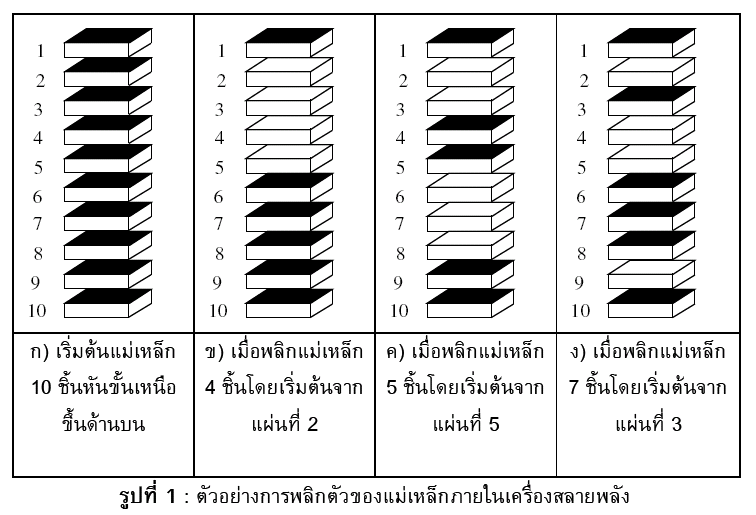
\includegraphics[width=0.7\textwidth]{../latex/img/1029/1029-1.png}
\end{figure}


ตัวอย่างการการพลิกแม่เหล็กสามารถแสดงได้ดังรูปที่ 1 สมมติให้มีแม่เหล็กทั้งสิ้น $10$ แผ่น และศาสตราจารย์เอ็กซ์ได้สั่งให้แขนกลพลังลมพลิกแม่เหล็กนี้ทั้งสิ้น $3$ ครั้ง โดยครั้งที่ $1$ จะพลิกแม่เหล็กจำานวน $4$ แผ่นเริ่มต้นจากแผ่นที่ $2$, ครั้งที่ $2$ พลิกแม่เหล็กจำนวน $5$ แผ่นเริ่มต้นจากแผ่นที่ $4$, และครั้งสุดท้ายพลิกแม่เหล็กเริ่มต้นจากแผ่นที่ $3$ เป็นจำนวน $7$ แผ่น

\bigskip
\underline{\textbf{โจทย์}}  จงเขียนโปรแกรมเพื่อหาว่าเมื่อหยุดการทำางานของเครื่องสลายพลังแม่เหล็ก ภายหลังจากการพลิกแม่เหล็กไปมาแล้วนั้น ถ้าต้องการหยิบแม่เหล็กขึ้นมาแผ่นหนึ่งจะมีแม่เหล็กที่ติดกับมันออกมาด้วยกี่ชิ้น


\InputFile

\textbf{บรรทัดแรก} รับจำนวนเต็ม $3$ จำนวน $N$ $M$ $Q$  แทนจำนวนแม่เหล็กทั้งหมด $(1 \leq N \leq 100\,000\,000)$ ,จำนวนครั้งที่พลิก $(1 \leq M \leq 100\,000)$ และจำนวนคำถาม $(1 \leq Q \leq 100\,000)$

\textbf{บรรทัดที่ $2$ ถึง $M+1$} บรรทัดที่ $i+1$ ให้รับข้อมูลการพลิกแม่เหล็กครั้งที่ $i$ โดยแต่ละบรรทัดจะรับข้อมูลจำนวนเต็มสองจำนวน $a$ $k$ แทนตำแหน่งเริ่มต้นของแม่เหล็กที่จะพลิก $(1 \leq a \leq N)$ และจำนวนชิ้นของแม่เหล็กที่พลิก $(1 \leq k \leq N)$ รับประกันว่าจะไม่พลิกแม่เหล็กเกินขอบเขตที่เป็นไปได้ กล่าวคือรับประกันว่า $1 \leq a+k-1 \leq N$

\textbf{บรรทัดที่ $M+2$ ถึง $M+Q+1$} บรรทัดที่ $M+i+1$ ให้รับข้อมูลคำถามที่ $i$ โดยในแต่ละบรรทัดจะรับข้อมูลตัวเลขเพียงจำนวนเดียว $x$ $(1 \leq x \leq N)$ แสดงถึงหมายเลขของแม่เหล็กที่ต้องการถาม

\OutputFile

\textbf{มี $Q$ บรรทัด} แต่ละบรรทัดให้แสดงจำนวนของแม่เหล็กทั้งหมดที่จะถูกหยิบออกมาเมื่อคุณหยิบแม่เหล็กแผ่นที่ถาม



\Examples

\begin{example}
\exmp{10 3 2
2 4
4 5
3 7
7
5}{3
2}%
\end{example}


\Source

Young Thai Online Programming Competition 2008

\end{problem}

\end{document}